\chapter{Hardware Developed}
During the development of this thesis there was both hardware and software developed. In this chapter we are going to go through the hardware developed in order to build an appropriate \acrfull{soc} capable of running a full-fledged \acrfull{os}.

The \textit{IOb-SoC} was used as a \acrfull{soc} template. \textit{IOb-SoC} has some features that make it ideal to develop this project \acrshort{soc}. Firstly it is open-source hardware. Witch means there are no royalties and the source code is publicly available. Secondly, adding new peripherals is very easy and intuitive, as it was previously seen in section \ref*{section:the_iob_soc_template}. Finally, it already has some features that make it ideal to use. \textit{IOb-SoC} already implements the interface with an internal (SRAM) and an external (DRAM) memory, contains iob-cache system and boot hardware unit. The boot hardware unit controls the first boot stage (also known as stage zero) that is executed after powering/resetting the system.

The hardware components that needed to be changed from \textit{IOb-SoC} were the \acrfull{cpu} and the \acrfull{uart} peripheral. The \acrshort{cpu} had to be changed because the previous \acrshort{cpu} (\textit{PicoRV32}) is not capable of running a full-feature \acrlong{os}. The \acrshort{uart} had to be swapped since there were no compatible Linux drivers that worked with \textit{iob-UART}. Besides swapping a few components from the chip new hardware had to be added. The additional hardware is the \acrshort{clint} and the \acrshort{plic} both compatible with RISC-V specifications. The \acrshort{clint} was added to add timer and software interrupts to the \acrshort{soc}. The \acrshort{plic} was added to manage interrupts generated by other peripherals, as for example from the \acrshort{uart}. A sketch of the \acrshort{soc} developed can be seen in figure \ref{fig:bd_linux}.

\begin{figure}[!h]
    \centering
    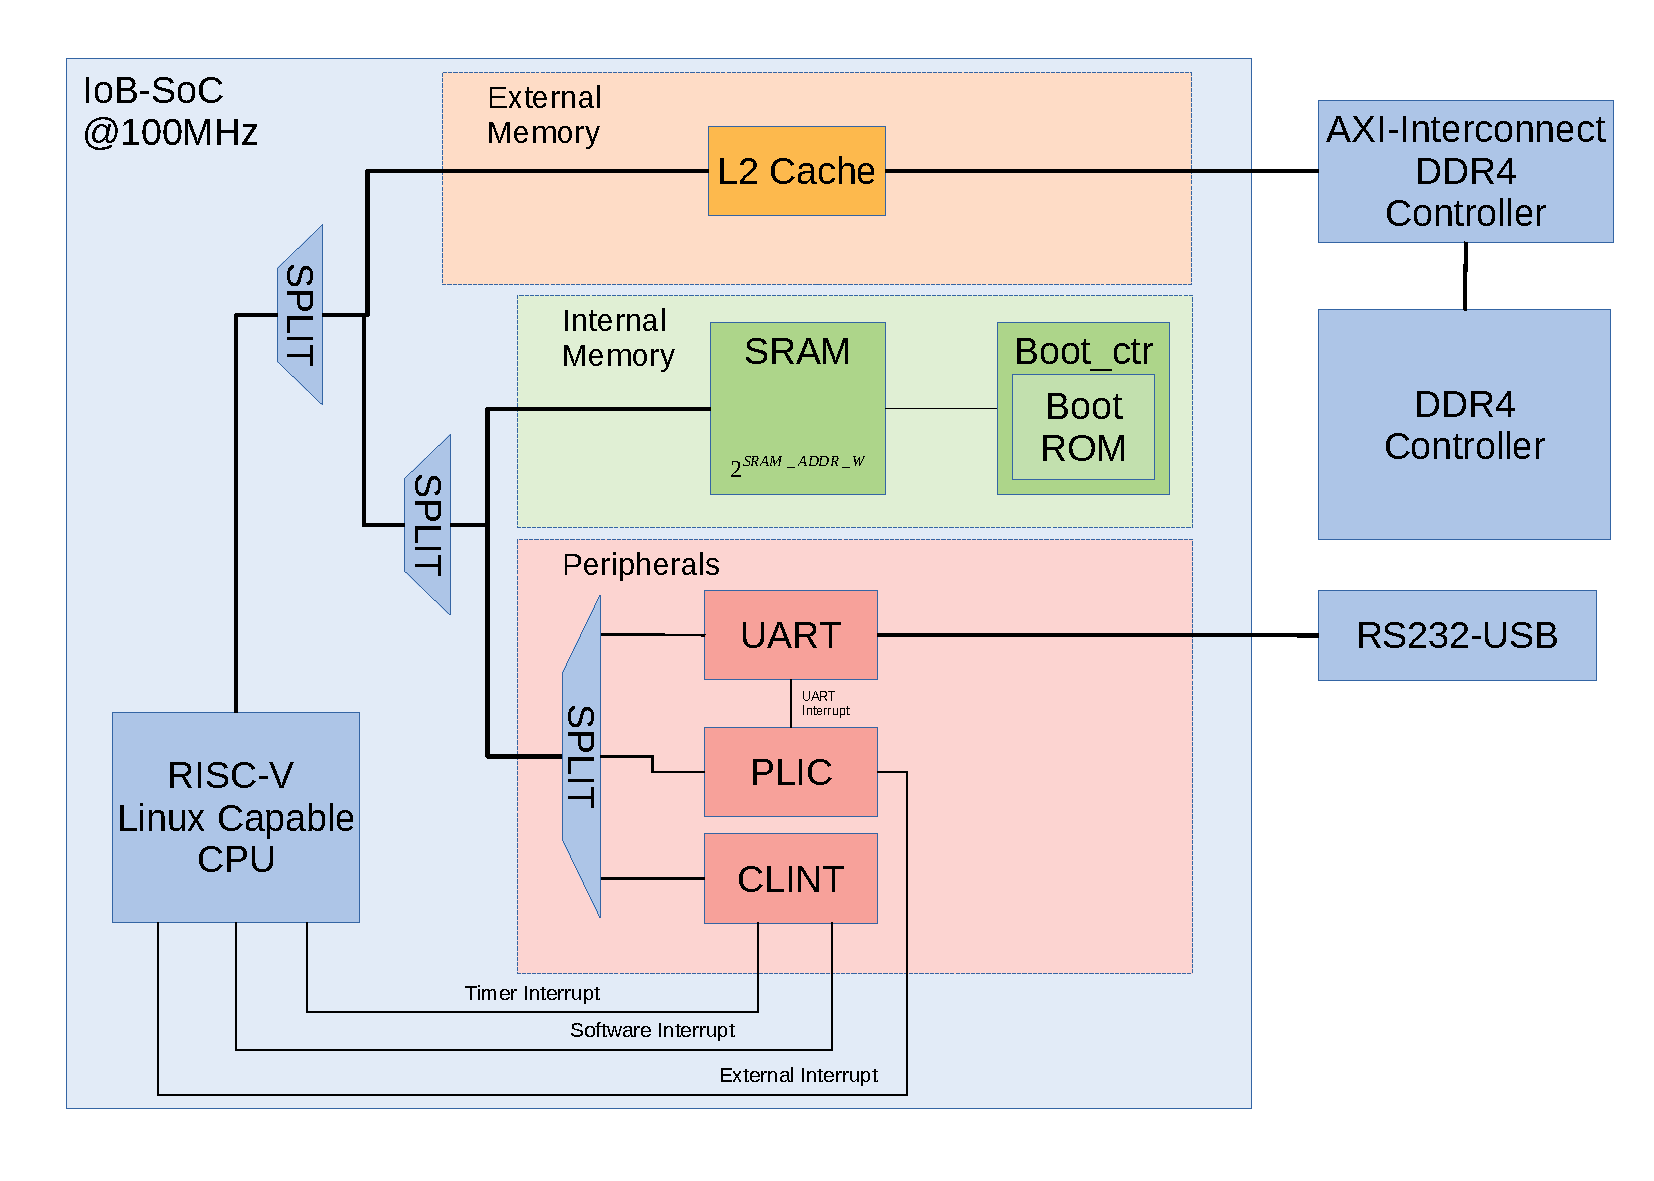
\includegraphics[width=0.7\linewidth]{bd_linux.pdf}
    \caption{Developed \acrshort{soc} sketch.}
    \label{fig:bd_linux}
\end{figure}

During this project there was also an improvement on the \textit{IOb-SoC} verification. This lead to the creation of a top hardware module for the developed \acrlong{soc}.

\section{Central Processing Unit}
The \acrshort{cpu} chosen to use in this project was \textit{VexRiscv}. \textit{VexRiscv} could be configured in various ways
\subsection{VexRiscv Wrapper}

\section{UART16550 Wrapper}
The approach taken in this project was to adapt an existing open-source UART core that is supported by the Linux kernel. The other option was to create a Linux driver compatible with \textit{iob-UART} and compile the kernel with it. The chosen approach seamed more adequate and simpler solution.

\section{CLINT Unit}
\acrshort{clint}

\section{PLIC Unit Wrapper}
\acrshort{plic} 

\section{UUT Top Hardware}
This top module creates a verilog wrapper of the \acrfull{uut} that allows it to interact with the different hardware logic simulators. The top module file is an adaptation of the previous verilog file used on icarus simulation.

\begin{figure}[!ht]
    \centering
    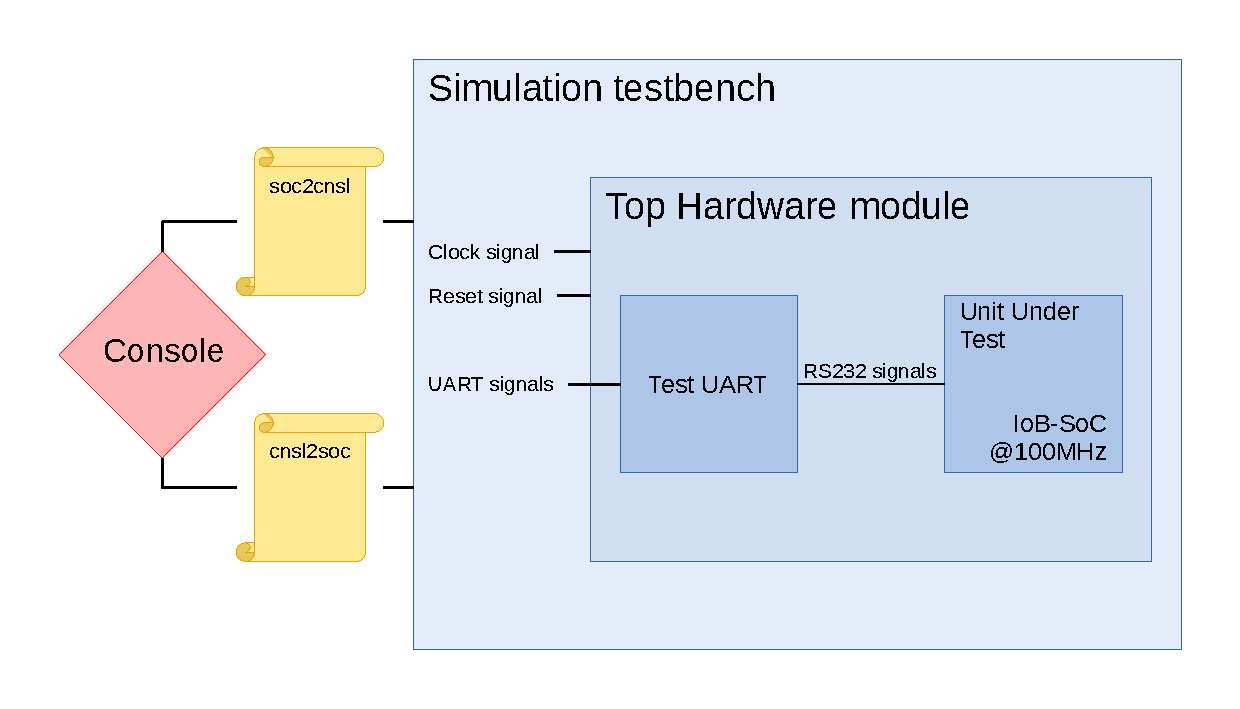
\includegraphics[width=\linewidth]{uut_top_hw.pdf}
    \caption{Simulated hardware interfaces.}
    \label{fig:uut_top_hw}
\end{figure}